% owner: jeffrey

\chapter{Projektzeitplan und Zuständigkeiten}
\label{cha:proz}

\begin{longtable}[h]{| l | l | l | p{7.5cm} |}
\hline
\bf{Id} & \bf{Fertigstellung} & \bf{Verantwortung} & \bf{Beschreibung}\\
\hline\hline
\endfirsthead
\multicolumn{4}{|c|}{\bf{Milestone 1: Anforderungsanalyse und -definition}}\\
\hline
AP1.1 & 21sep2010 & TST & Analyse der vorhandenen Software\\
AP1.2 & 23sep2010 & TST & Anforderungsbesprechung mit Kunde\\
AP1.3 & 05okt2010 & TST & Fertigstellung CRS, Präsentation\\
AP1.4 & 07okt2010 & TST,DH & Präsenation CRS beim Kunden\\
GATE1.5 & 08okt2010 & - & Abnahme CRS durch Kunden\\
AP1.6 & 01nov2010 & DH,JJ,KW,TST & Fertigsgtellung SRS\\
AP1.7 & 15nov2010 & TST,JJ & Präsentation SRS\\
GATE1.8 & 16nov2010 & - & Abnahme SRS durch Kunden\\
\hline
\multicolumn{4}{|c|}{\bf{Milestone 2: Systementwurf}}\\
\hline
AP2.1 & 11okt2010 & JJ & Festlegung zu verwendender Komponenten und
Technologien\\
AP2.2 & 20okt2010 & JJ,KW & Entwurf der Systemarchitektur\\
AP2.3 & 25okt2010 & JJ,KW & Definition von Systemkomponenten\\
AP2.4 & 12nov2010 & DH & Zuweisung Arbeitspakete an Bearbeiter\\
AP2.5 & 12nov2010 & KW & Fertigstellung SAS\\
GATE2.6 & 12nov2010 & DH,TST,JJ,KW & Abnahme von SAS durch Projektleiter,
Produktmanager sowie den leitenden Ingenieuren\\
\hline
\multicolumn{4}{|c|}{\bf{Milestone 3: Implementierung}}\\
\hline
AP3.1 & 20nov2010 & JJ & Anpassung der Arbeitspakete an Entwicklungsmodell sowie
unterstützendes Tooling\\
AP3.2 & 15feb2011 & separat & Fertigstellung: Implementierung der
Systemkomponenten\\
AP3.3 & 28feb2011 & RS & Fertigstellung: Dokumentation der Systemkomponenten\\
GATE3.4 & 02mar2011 & - & Abnahme der Module durch Projektleiter,
Produktmanager sowie den leitenden Ingenieuren\\
\hline
\multicolumn{4}{|c|}{\bf{Milestone 4: Systemintegration und Test}}\\
\hline
AP3.4 & 28feb2011 & JJ,KW &Zusammenführung des Gesamtsystems\\
AP4.1 & 18mar2011 & TSC & Abschluss aller Komponententests und Testberichte\\
AP4.2 & 25mar2011 & TSC,JJ,KW & Auswertung der Testberichte\\
AP4.3 & 17apr2011 & JJ,KW & Verfeingerung, Bugfixing\\
AP4.4 & 28apr2011 & TSC & finaler Testbericht\\
GATE4.5 & 30apr2011 & JJ,KW & Abnahme Gesamtsystem inkl. Testbericht durch
leitende Ingenieure\\
\hline
\multicolumn{4}{|c|}{\bf{Milestone 5: Übergabe und Einführung}}\\
\hline
AP5.1 & 01may2011 & TSC & Optimierung und Fertigstellung der
Systemdokumentation\\
AP5.2 & 03may2011 & JJ & Deploymentmethode wählen und realisieren\\
AP5.3 & 03may2011 & TST & Präsentation des Endproduktes fertigstellen\\
AP5.4 & 06may2011 & TST & Produktpräsentation und Übergabe\\
GATE5.5 & 06may2011 & - & Produktabnahme durch Kunde\\
AP5.6 & 15may2011 & TST & Schulungswünsche mit Kunde klären\\
AP5.7 & 31may2011 & DH & Arbeitsaufwände in Rechnung stellen\\
\hline
\caption{Milestone-Liste}
\end{longtable}

\clearpage

\begin{landscape}
\begin{figure}
\centering
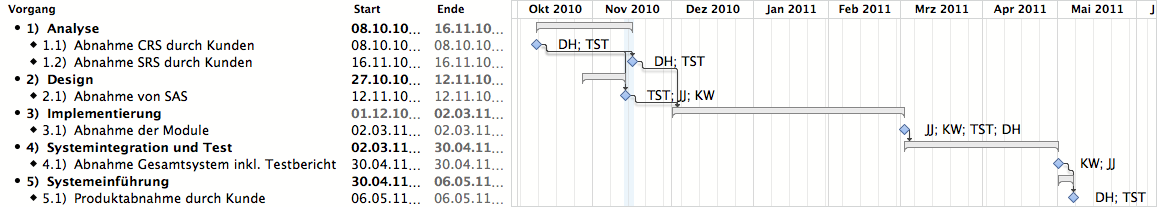
\includegraphics[width=22cm]{images/Projekt-Gantt.png}
\caption{Gantt-Diagramm}\label{fig:gantt}
\end{figure}
\end{landscape}

\chapter{Modulzeitplan und Zuständigkeiten}
\label{cha:modu}
Während der Designphase wurden die folgenden Module identifiziert:

\begin{table}[h]
\caption{Module und Zuständigkeiten}
\label{tab:modz}
\begin{center}
\begin{tabular}{|l|c|p{8cm}|}
\hline
\textbf{Modulname} & \textbf{Verantwortung} & \textbf{Beschreibung}\\
\hline
GUI-Design & TST & Design der grefischen Benutzer Oberfläche\\
\hline
GUI-Logik & TSC & Logik, die hinter der Gui steckt. Konfiguration, Aktualisierung, Listener.\\
\hline
Controller/Profile & DH & Entwicklung des Controllers inklusive der Profil-Verwaltung, Speicherung und dem Laden.\\
\hline
CLI/Logger & RS & Entwicklung der Konsolenschnitstelle inklusive des Loggers.\\
\hline
Sender/Receiver & JJ & Multicast Sende/Empfangsmöglichkeit inklusive der Verwaltung und der Logik.\\
\hline
Paket & KW & Paketdesign und Implementierung.\\
\hline
Language & KW & Entwurf und Verwaltung der Spracheinstellungen.\\
\hline
Installer & KW & Einfache Installation auf Windows und unter Linux Debian.\\
\hline
\end{tabular}
\end{center}
\label{default}
\end{table}

\clearpage

\begin{landscape}

Die Startzeiten sind je nach Fertigstellung der Arbeitspakete noch variabel. Die Endzeiten sind jedoch fix und müssen unbedingt eingehalten werden.
\begin{table}[h]
\caption{Modulzeitplan}
\label{tab:modz}
\begin{center}
\begin{tabular}{|l|c|c|c|c|c|c|}
\hline
\textbf{Modulname} & \textbf{Start} & \textbf{Ende} & \textbf{Zeit Design} & \textbf{Zeit Impl.} & \textbf{Zeit Integration und Test} & \textbf{Zeit Ges.}\\
\hline
GUI-Design & 01dez2010 & 20jan2011 & 2 MT & 8 MT & 5 MT & 15 MT\\
\hline
GUI-Logik &  01dez2010 & 30jan2011 & 3 MT & 8 MT & 6 MT & 17 MT\\
\hline
Controller/Profile &  01dez2010 & 20jan2011 & 3 MT & 8 MT & 5 MT & 16 MT\\
\hline
CLI/Logger &  01dez2010 & 30jan2011 & 2 MT & 8 MT & 3 MT & 13 MT\\
\hline
Sender/Receiver & 01dez2010 & 10jan2011 & 6 MT & 9 MT & 7 MT & 22 MT\\
\hline
Paket & 01dez2010 & 01jan2011 & 2.5 MT & 4 MT & 6 MT & 12.5 MT\\
\hline
Language &  01jan2010 & 20jan2011 & 0.5 MT & 4 MT & 4 MT & 8.5 MT\\
\hline
Installer &  28jan2010 & 10feb2011 & 1 MT & 4 MT & 2 MT & 7 MT\\
\hline
\textbf{Gesamt} & \textbf{01dez2010} & \textbf{10feb2011} & \textbf{20 MT} & \textbf{53 MT} & \textbf{38 MT} & \textbf{111 MT}\\
\hline
\end{tabular}
\end{center}
\label{default}
\end{table}
\end{landscape}

\clearpage

\begin{landscape}
\begin{figure}
\centering
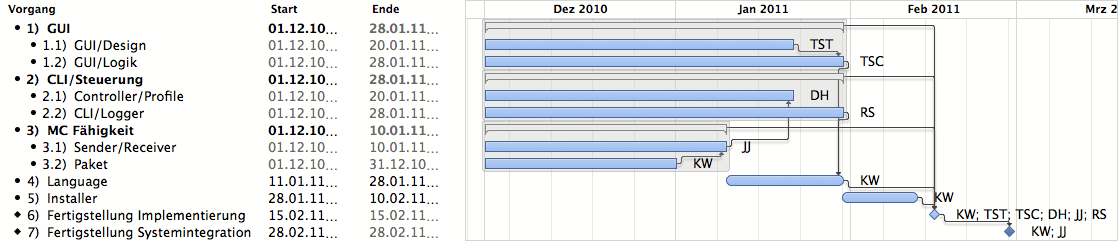
\includegraphics[width=22cm]{images/Modul-Gantt.png}
\caption{Gantt-Diagramm}\label{fig:gantt}
\end{figure}
\end{landscape}

\begin{figure}[h]
\centering
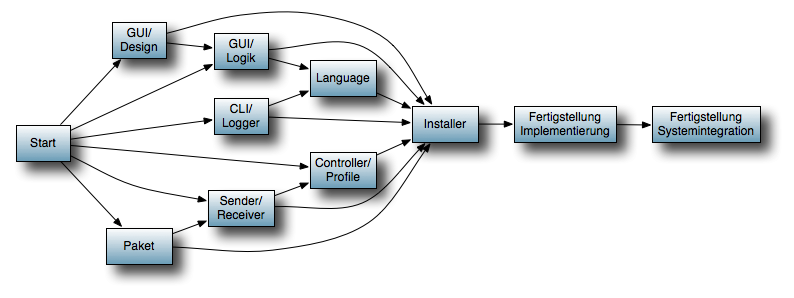
\includegraphics[width=16.5cm]{images/Modul-Netz.png}
\caption{Modul-Implementierung Netzdiagramm}\label{fig:modulnetz}
\end{figure}

Die beiden GUI Module besitzen eine Ende-zu-Ende Abhängigkeit.\\
Sender/Receiver und Controller/Profile besitzen eine Ende-zu-Ende Abhängigkeit und müssen viel wärend der Entwicklung zusammenarbeiten.\\
Sender/Receiver und Paket besitzen eine Ende-zu-Ende Abhängigkeit und müssen sich wärend der Entwicklung abstimmen.\\
GUI-Design und Language besitzen eine Ende-zu-Ende Abhängigkeit.\\
CLI/Logger und Language besitzen eine Ende-zu-Ende Abhängigkeit.\\
Installer besitzt eine Ende-zu-Ende Abhängigkeit zu allen anderen Modulen.\\
